 \documentclass[a4paper,12pt]{report}

%Packages Used
\usepackage{amssymb,latexsym,amsmath}     % Standard packages
\usepackage{setspace}
\usepackage{sectsty}
\usepackage{titlesec}
\usepackage{hyperref}
\usepackage{bookmark}
\usepackage{graphics,graphicx}
\usepackage{tikz}
\usepackage{mathtools}
\usepackage{graphicx}
\usepackage{esvect}

\DeclarePairedDelimiter\abs{\lvert}{\rvert}%
\DeclarePairedDelimiter\norm{\lVert}{\rVert}%


\bookmarksetup{
  numbered,
  open
}
\renewcommand*{\thesection}{\arabic{section}}
\onehalfspacing

%Margins
\addtolength{\textwidth}{1.0in}
\addtolength{\textheight}{1.00in}
\addtolength{\evensidemargin}{-0.75in}
\addtolength{\oddsidemargin}{-0.75in}
\addtolength{\topmargin}{-.50in}

%%%%%%%%%%%%%%%%%%%%%%%%%%%%%% 
% Theorem/Proof Environments %
%%%%%%%%%%%%%%%%%%%%%%%%%%%%%%
\newtheorem{theorem}{Theorem}
\newenvironment{proof}{\noindent{\bf Proof:}}{$\hfill \Box$ \vspace{10pt}}
\sectionfont{\fontsize{12}{15}\selectfont}
\titlespacing*{\section}{0.5pt}{0.25\baselineskip}{0.25\baselineskip}

\begin{document}
\noindent
Yufei Lin

\noindent
Advance Computer Graphic Final

\noindent
Nov \(21^{th}\) 2019

\begin{center}
\textbf{Torus Primitive}
\end{center}

Torus is one of the most important shape in our life. We have bagels, doughnuts and many other things. In order to have a better reconstruction of our daily life scenes in a 3D renderer, the best way to introduce torus as a single primitive instead of a combination of triangles or any other shapes. 

\begin{figure}[h]
\centering
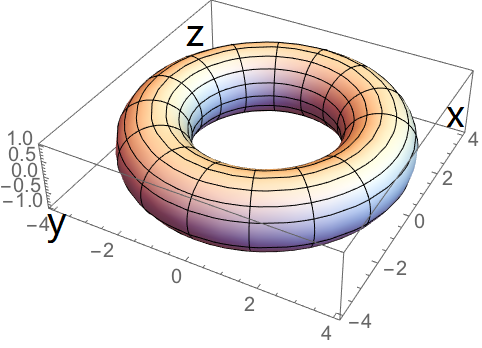
\includegraphics[scale=1]{./Pic/Torus1.png}
\caption{Torus Perspective View}
\end{figure}

\noindent
\textbf{I. Defining a Torus}

There are three circles in a torus $C_1, C_2, C_3$ as shown in the graph below. $C_2$ is how a torus is defined, because the center of the tube is uniformly lying on it and by utilizing it we can reduce our equation for the torus.  Then, we have the radius of $C_2$ as $R$ and the raidus of the tube as $r$. Therefore, we know that from this graph:
\(x^2+y^2=R^2\).
\begin{figure}[h]
\centering
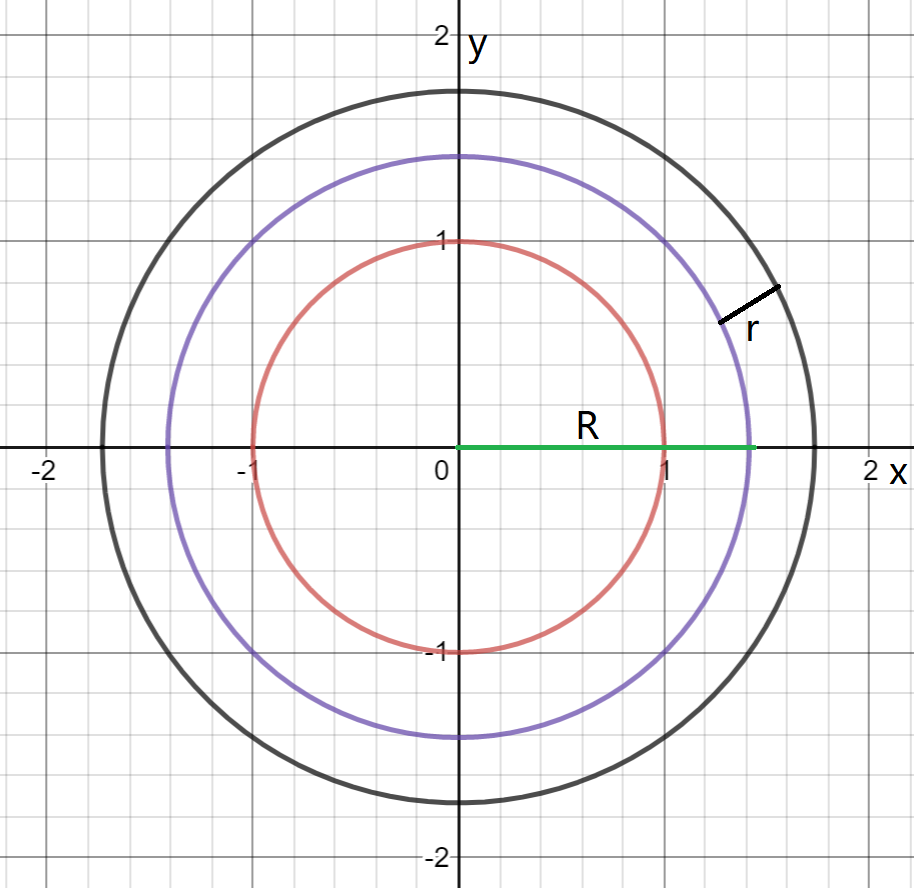
\includegraphics[scale=0.4]{./Pic/Torus2.png}
\caption{Torus Top View}
\end{figure}

Then, we just need to obtain the torus from $x,y$ and $z$. Based on observation, we can see the cross section of a torus as the following graph, and could interpret that the size of the cube should be a function like the following: $(g(x,y))^2+z^2=r^2$. This means 
\begin{figure}[h]
\centering
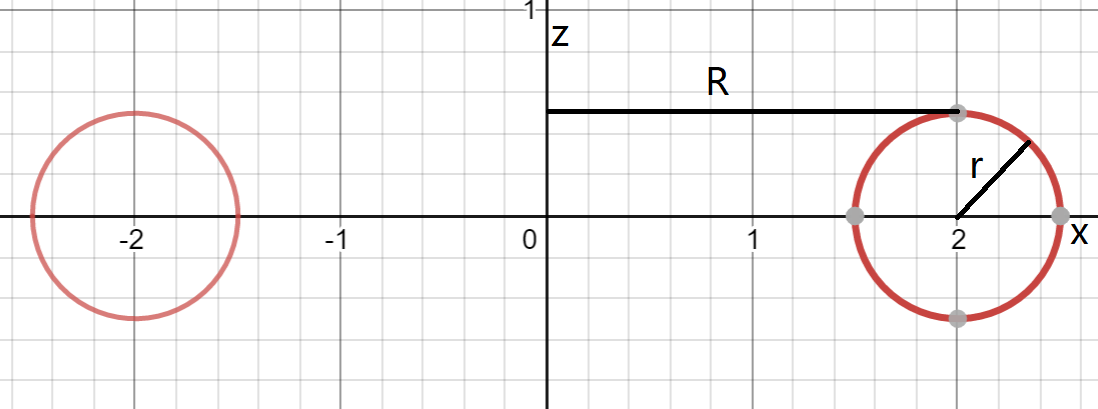
\includegraphics[scale=0.4]{./Pic/Torus3.png}
\caption{Torus Top View}
\end{figure}


\end{document}